\documentclass{beamer}

\usepackage[czech]{babel}
\usepackage[utf8]{inputenc}
\usepackage[T1]{fontenc}
\usepackage{graphicx}
\usepackage{svg}
\usepackage{caption}

\let\oldfootnotesize\footnotesize
\renewcommand*{\footnotesize}{\oldfootnotesize\small}

\setbeamertemplate{navigation symbols}{}
% \setbeamertemplate{logo}{
\includegraphics[width=2cm]{soc/images/spsejecna_logo.pdf}}

\title{FWKES}
\subtitle{Emulace hardwaru na příkladu herní konzole NES na~mikrokontroléru RP2350}
\author{Alexey Kachaev, Jakub Jansa}
\institute{Střední průmyslová škola elektrotechnická, Praha 2, Ječná 30}
\date{2026}

\titlegraphic{\hfill\hspace{1cm}\vspace{-2cm}
\includegraphics[width=5cm]{soc/images/spsejecna_logo.pdf}}

\begin{document}

\begin{frame}[plain]
\titlepage

% \begin{tikzpicture}[remember picture, overlay]
% \node[anchor=south east] at ([xshift=-0.5cm,yshift=0.5cm]current page.south east)
%     {
\includegraphics[width=3cm]{soc/images/spsejecna_logo.pdf}};
% \end{tikzpicture}

\end{frame}

% \frame{\titlepage}

\begin{frame}
\frametitle{Obsah}
\tableofcontents
\end{frame}

\section{Úvod}

\begin{frame}
\frametitle{Cíl}

\begin{itemize}
    \item \textbf{Návrh a realizace emulátoru} herní konzole Nintendo Entertainment System
        (NES).
    \item Cílem není jen hraní her, ale hlavně \textbf{pochopení a implementace} původního
    hardwaru, a \textbf{opětovné využití} získaných znalostí. Je to jen \textbf{demonstrační prvek}.
    \item Náš emulátor je schopen \textbf{přímo}
        vykonávat původní ROM obrazy\footnote{ROM obraz je obsah ROM pamětí, převedený do snadno
        přenositelné podoby (např. jako soubor). V případě NESu, obsahem je kód her a jejich data.}
        určené pro NES, a slušně opakuje originální zážitky.
\end{itemize}

\end{frame}

\section{Proč NES?}

\begin{frame}
\frametitle{Proč NES?}

\begin{columns}
    \column{0.5\textwidth}
    \begin{itemize}
        \item Velice známá a vlivná herní konzole 80. a 90. let, která zanechala kulturní stopy i
            dodnes.
        \item Ideální poměr mezi složitostí a rozsahem našeho projektu.
        \item Zdokumentovanost a obrovská komunita lidí, které stále mají zájem o konzoli, její
            architekturu a programování.
    \end{itemize}
    \column{0.5\textwidth}
    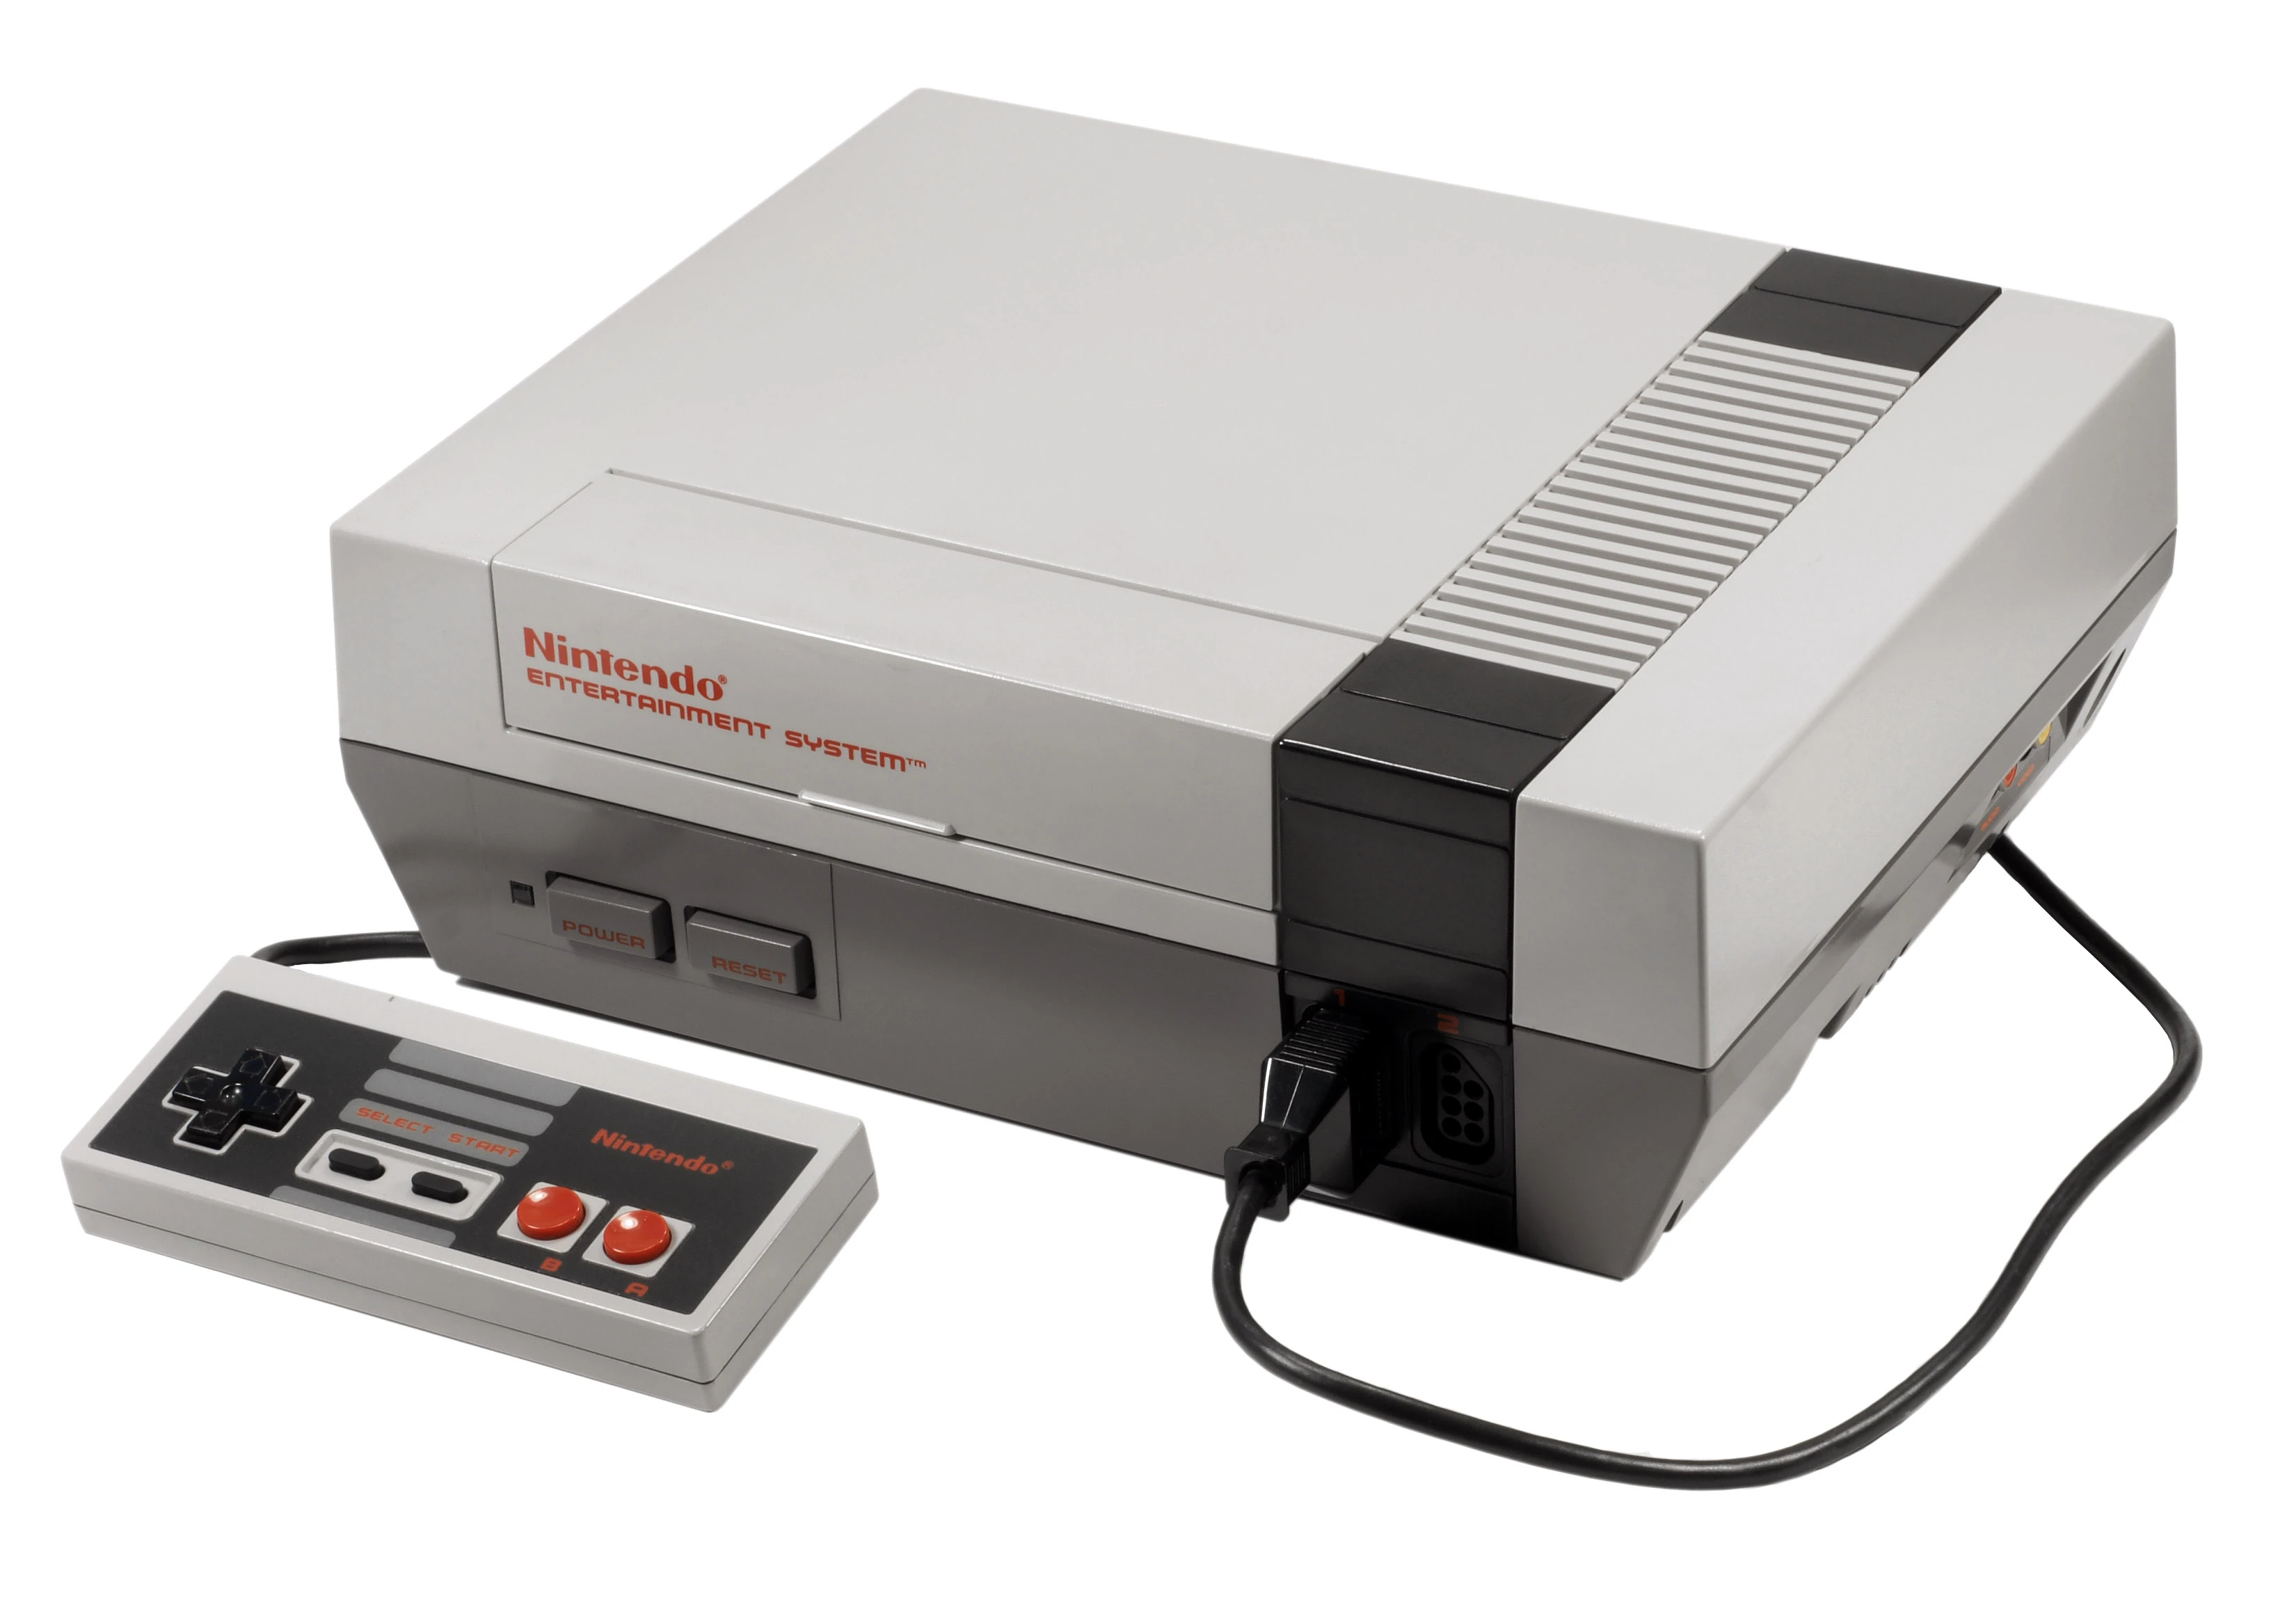
\includegraphics[width=1.0\textwidth]{images/nes.png}
    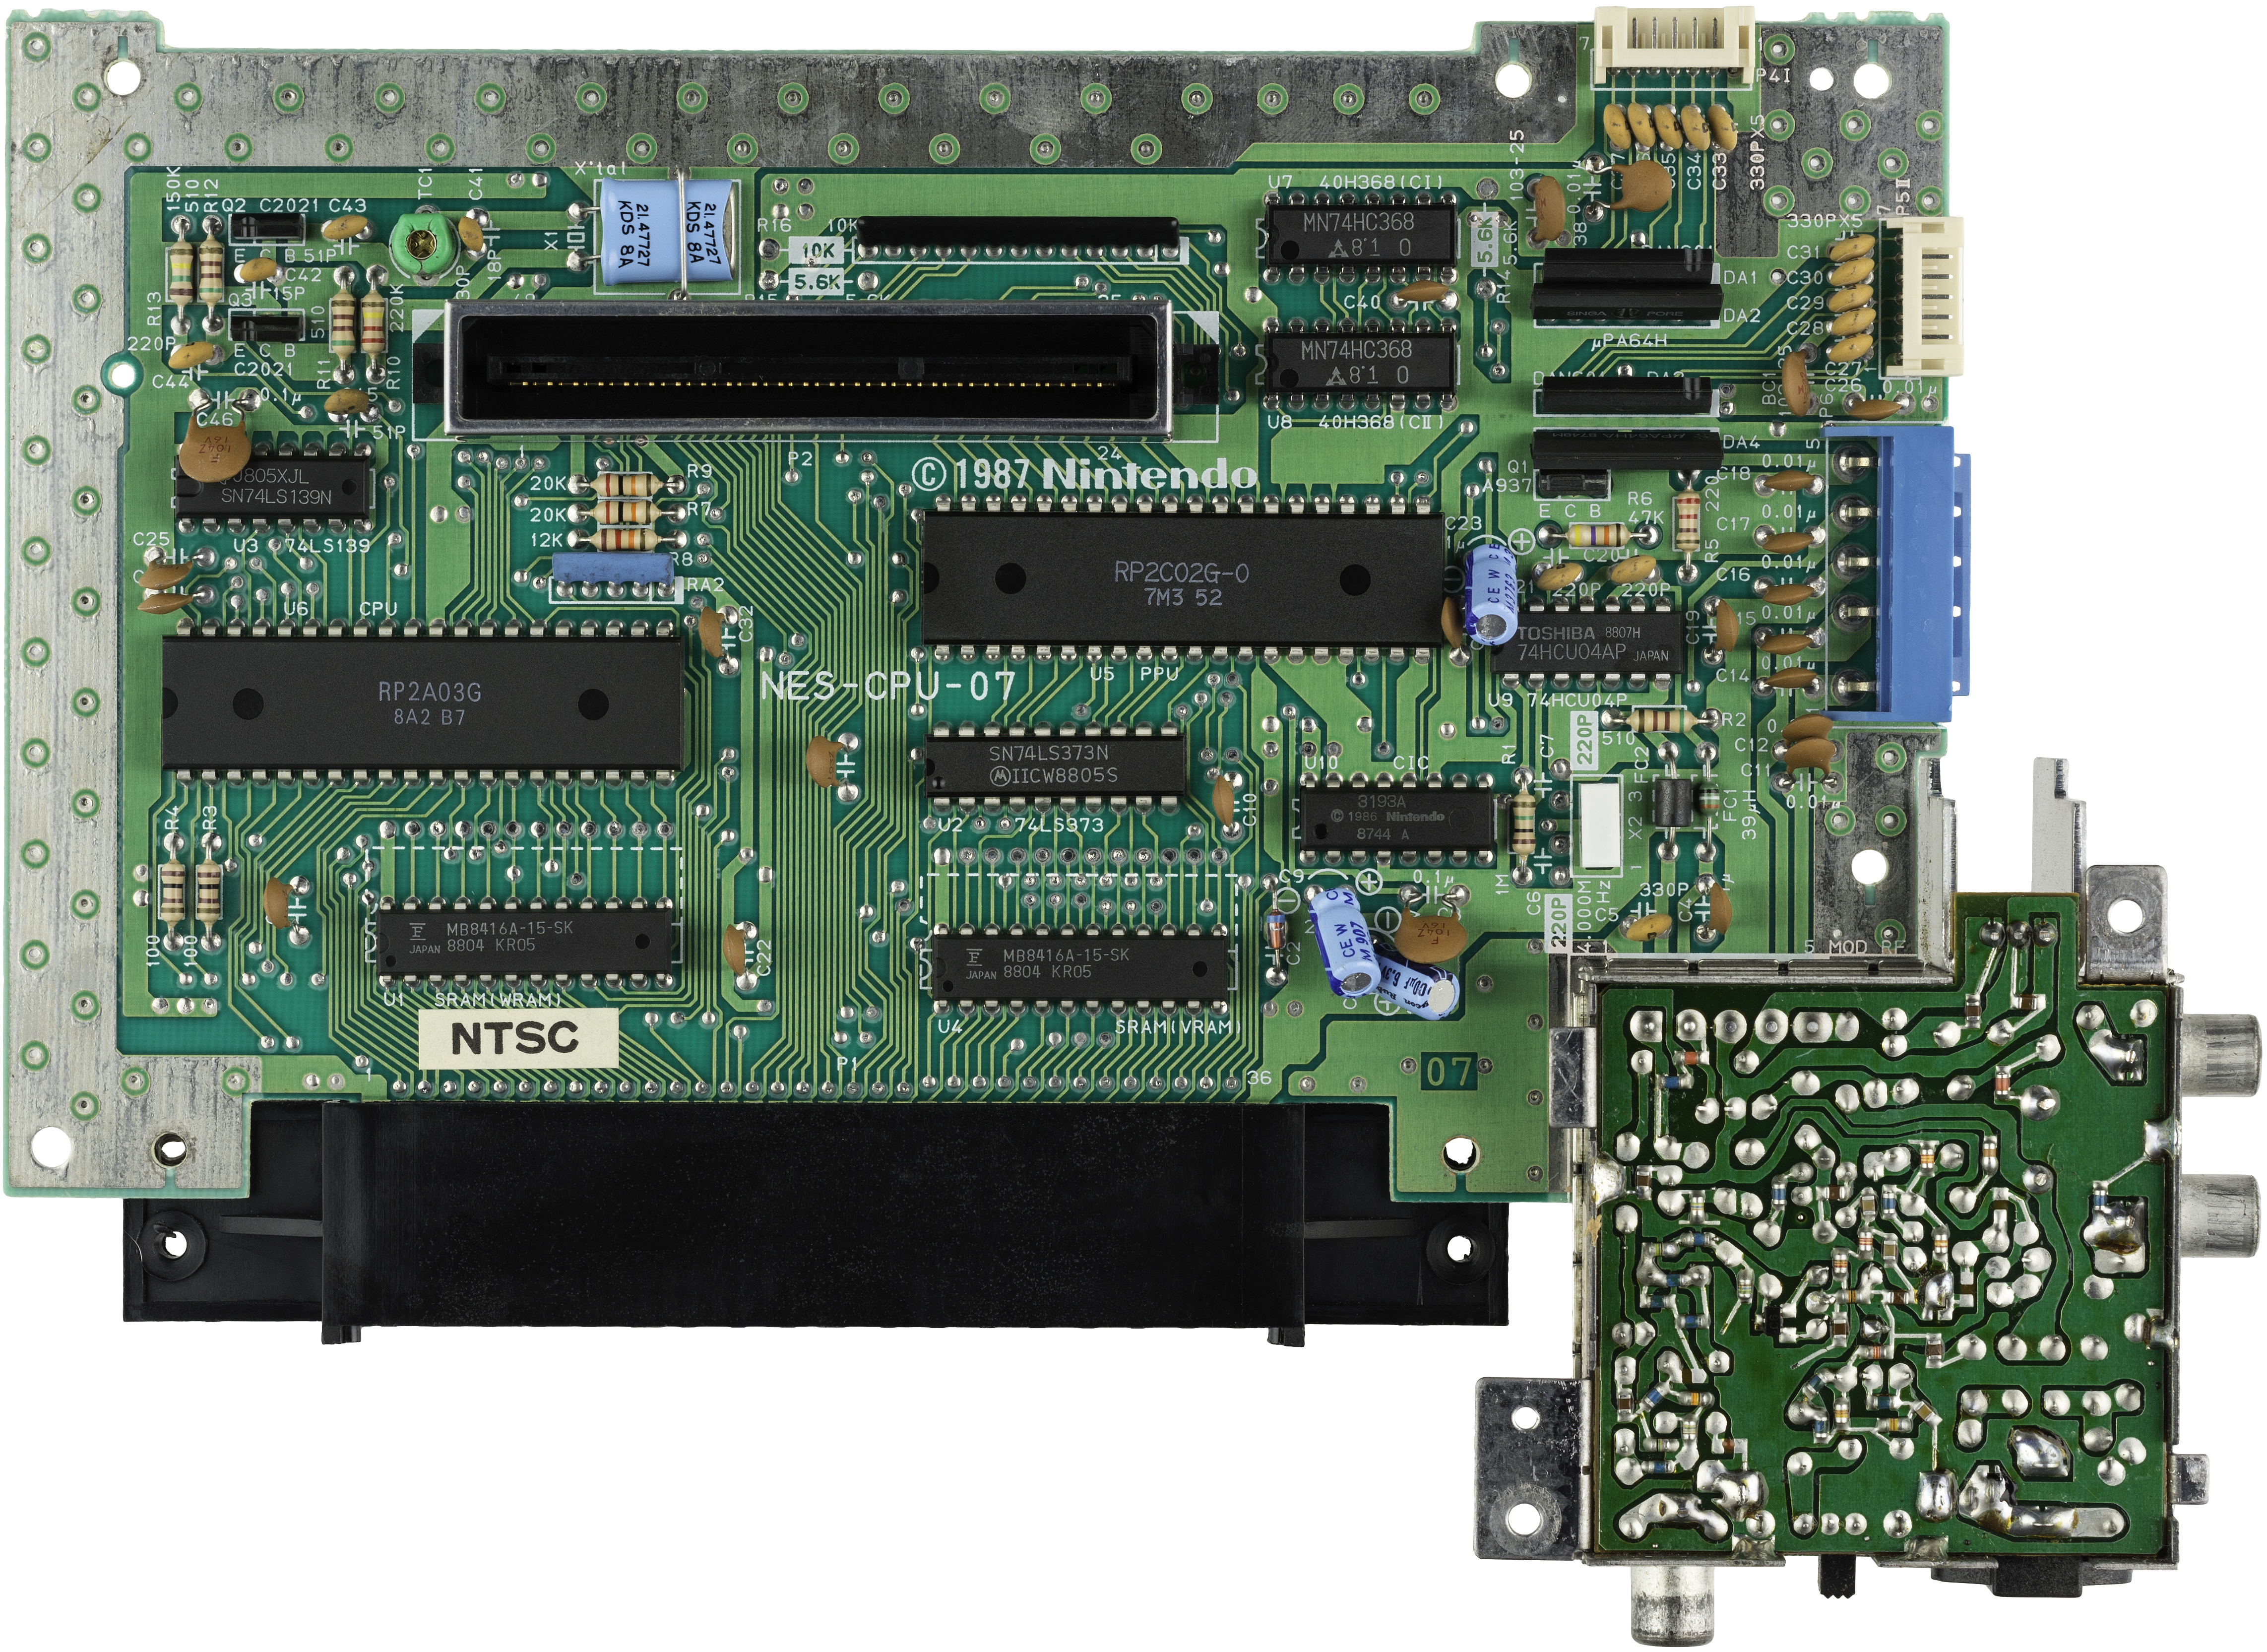
\includegraphics[width=0.75\textwidth]{images/nes_motherboard.jpg}
\end{columns}

\end{frame}

\section{Co je emulace?}

\begin{frame}
\frametitle{Co je emulace?}

\begin{itemize}
    \item Emulace je \textbf{napodobení chování} původního hardwaru, ne jen výsledku.
    \item CPU, paměť, grafika, a zvuk musí reagovat a spolupracovat stejně jako
        original.
    \item Program si ,,myslí'', že běží na původním systému.
    \item Emulace je přesná jen do určité míry.
    \item \emph{Je to způsob, jak porozumět hardwaru do hloubky -- nejen ho používat.}
\end{itemize}

\end{frame}

% \section{Proč je emulace obtížná}
%
% \begin{frame}
% \frametitle{Proč je emulace obtížná?}
%
% \begin{itemize}
%     \item Emulace je \textbf{reverzní inženýrství v praxi}: vyžaduje čtení velkého množství
%         dokumentace a experimentování.
%     \item Synchronizace komponentů systému.
%     \item Nižší úroveň emulace $\rightarrow$ vyšší nároky na výkon.
%     \item Případ NES:
%         \begin{itemize}
%             \item Přesné časování.
%             \item Každý komponent běžel samostatně, nezávisle od ostatních.
%             \item Programy využívaly nedokumentované chování.
%             \item Spousta úsporných řešení, které ztěžují celkové chápání systému.
%         \end{itemize}
%
%     % \item NES nebyl navržen pro emulaci:
%     %     \begin{itemize}
%     %         \item Přesné časování mezi jednotlivými komponenty.
%     %         \item Každý komponent běžel samostatně, nezávisle od ostatních.
%     %         \item Hry často využívaly chyby a nedokumentované chování.
%             % \item Omezený výkon a možností původního systému $\rightarrow$ spousta úsporných
%             %     řešení, které ztěžují celkové chápání systému.
%     %     \end{itemize}
% \end{itemize}
%
% \end{frame}
%
% \begin{frame}
%     \frametitle{Proč je emulace obtížná v \underline{našem} případě?}
%
%     \begin{itemize}
%         \item Většina počítačových emulátorů využívají výkonné procesory, grafické zrychlení,
%              velkou kapacitu RAM a prostředky OS.
%         \item RP2350 ale nedisponuje těmito možnostmi:
%             \begin{itemize}
%                 \item Žádný OS.
%                 \item Žádné GPU.
%                 \item  Nutnost ručně realizovat základní prostředky: souborový system,
%                     grafický výstup, zvukový výstup a vstup.
%                 \item 520 KB vestavěné RAM pamětí.
%                 \item Stabilní frekvenční rozsah je menší než 350 MHz.
%             \end{itemize}
%         \item Kompromis mezi přesnosti a rychlostí.
%     \end{itemize}
% \end{frame}

\section{Blokové schéma systému}

\begin{frame}
\frametitle{Blokové schéma systému}

\centering
\vspace{0.1cm}
\includesvg[width=0.9\textwidth]{soc/images/fwkes_architecture.svg}

\end{frame}

\section{Architektura emulátoru}

\begin{frame}
\frametitle{Architektura emulátoru}

\begin{itemize}
    \item CPU -- Central Processing Unit
    \item PPU -- Picture Processing Unit
    \item APU -- Audio Processing Unit
    \item Mapovací řadiče -- mappery
\end{itemize}

\centering
\includesvg[width=0.9\textwidth]{soc/images/memory_map_ex.svg}

\end{frame}

\section{Princip funkčností emulátoru}

\begin{frame}
\frametitle{Princip funkčností emulátoru}

\begin{itemize}
    \item \textbf{Doháněcí metoda} (\textit{catch-up method})
    \item CPU vykoná -- ostatní subsystémy doženou
    \item CPU přistupuje -- přistupováný subsystém dohání
\end{itemize}

\vspace{0.75cm}

\centering
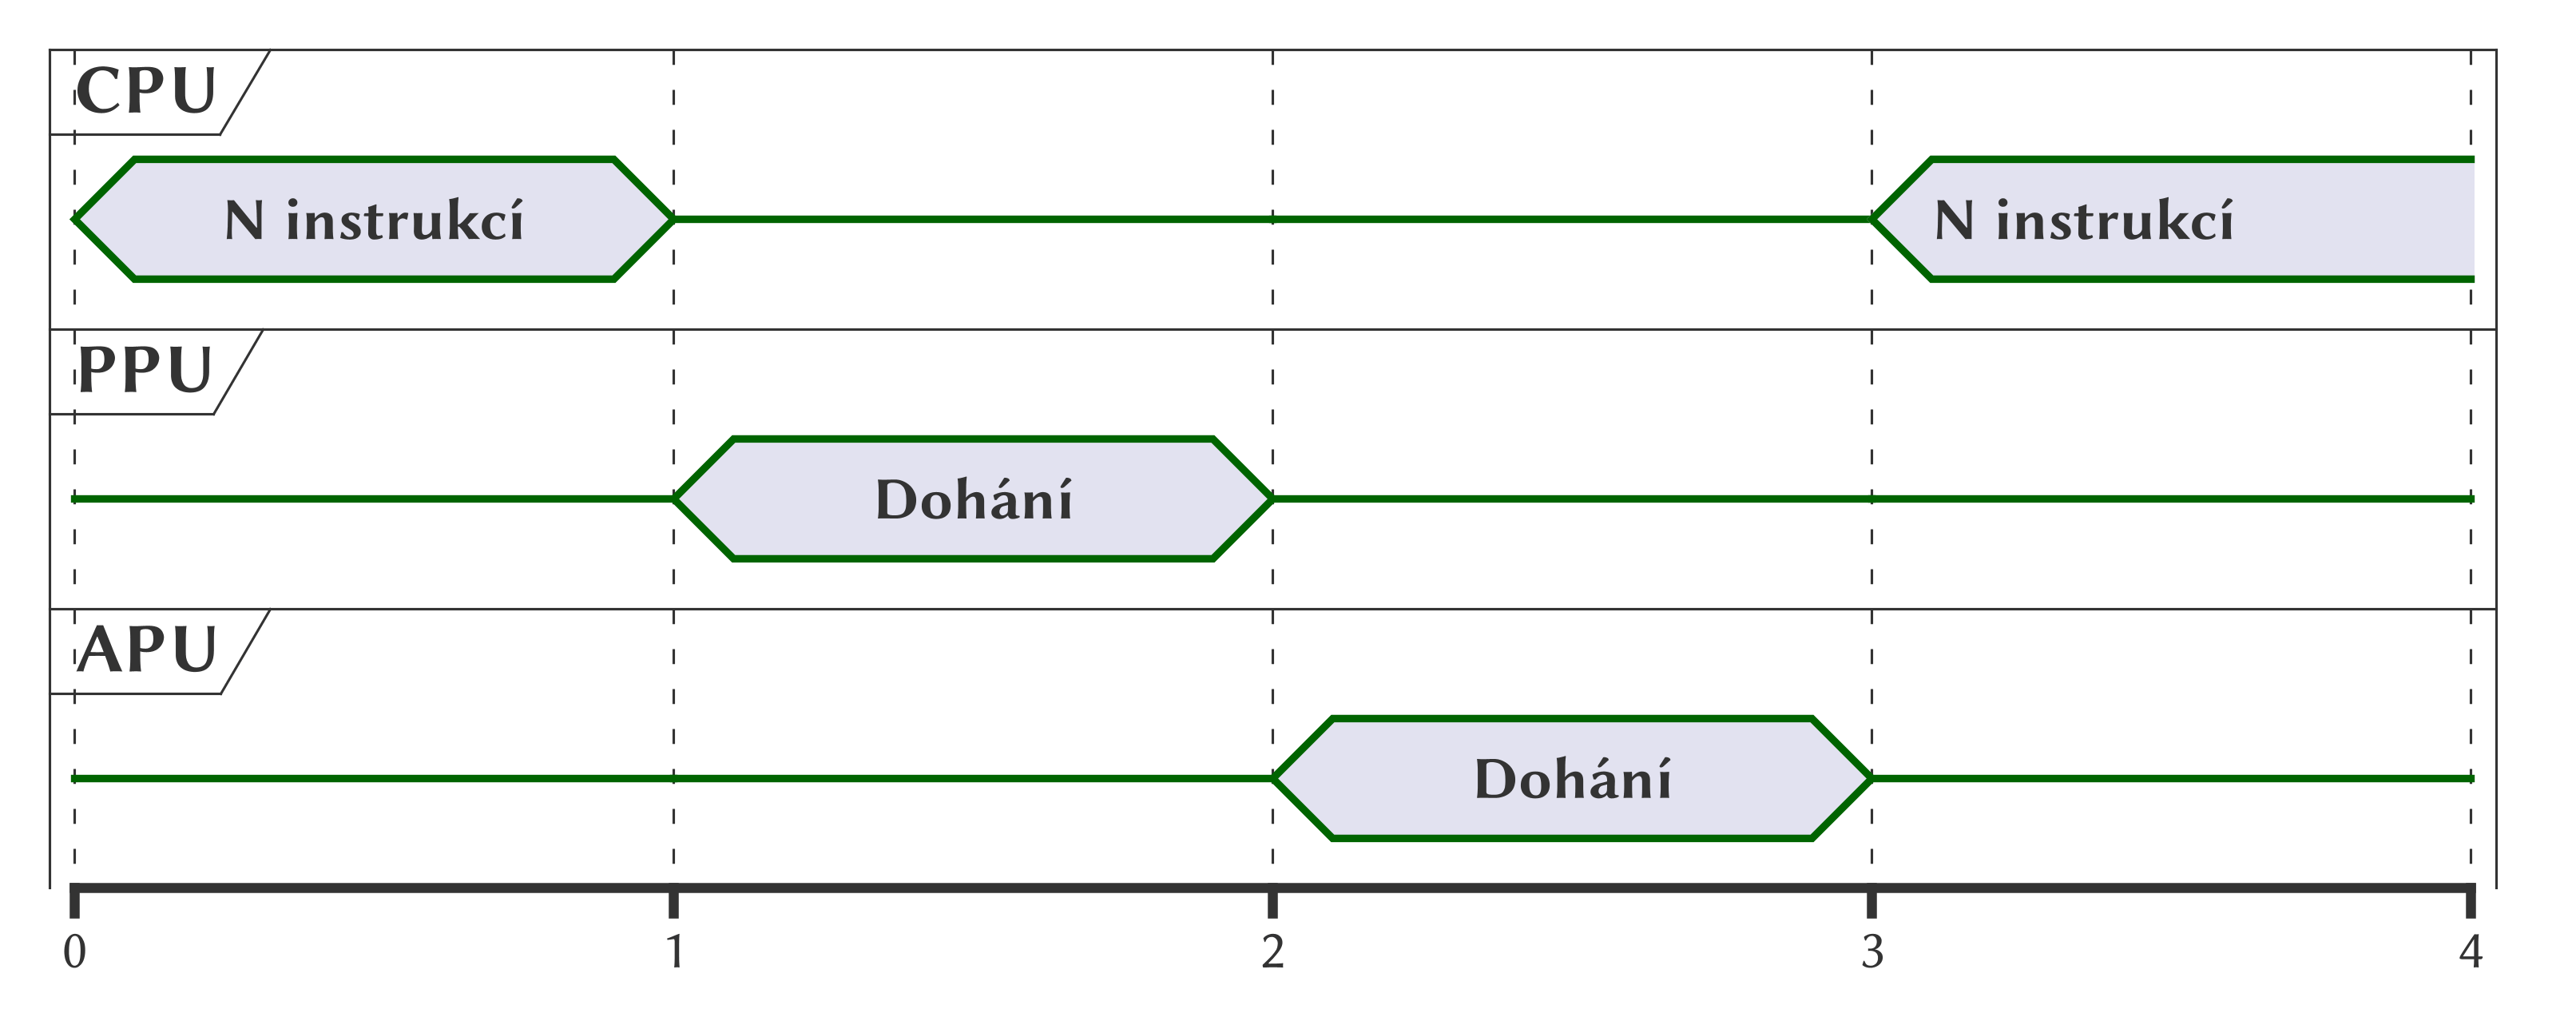
\includegraphics[width=\textwidth]{images/catch_up.png}

\end{frame}

\section{FWX (FirmWare eXchange)}

\begin{frame}
\frametitle{FWX (FirmWare eXchange)}

\begin{itemize}
    \item Komunikační datová linka
    \item Dovoluje vyjít za hranice NES $\rightarrow$ obecný počítač
    \item Momentálně: práce s SD kartou a načtení programu z SD karty
    \item V budoucnu: GPIO rozhraní a konfigurace zařízení
\end{itemize}

\centering
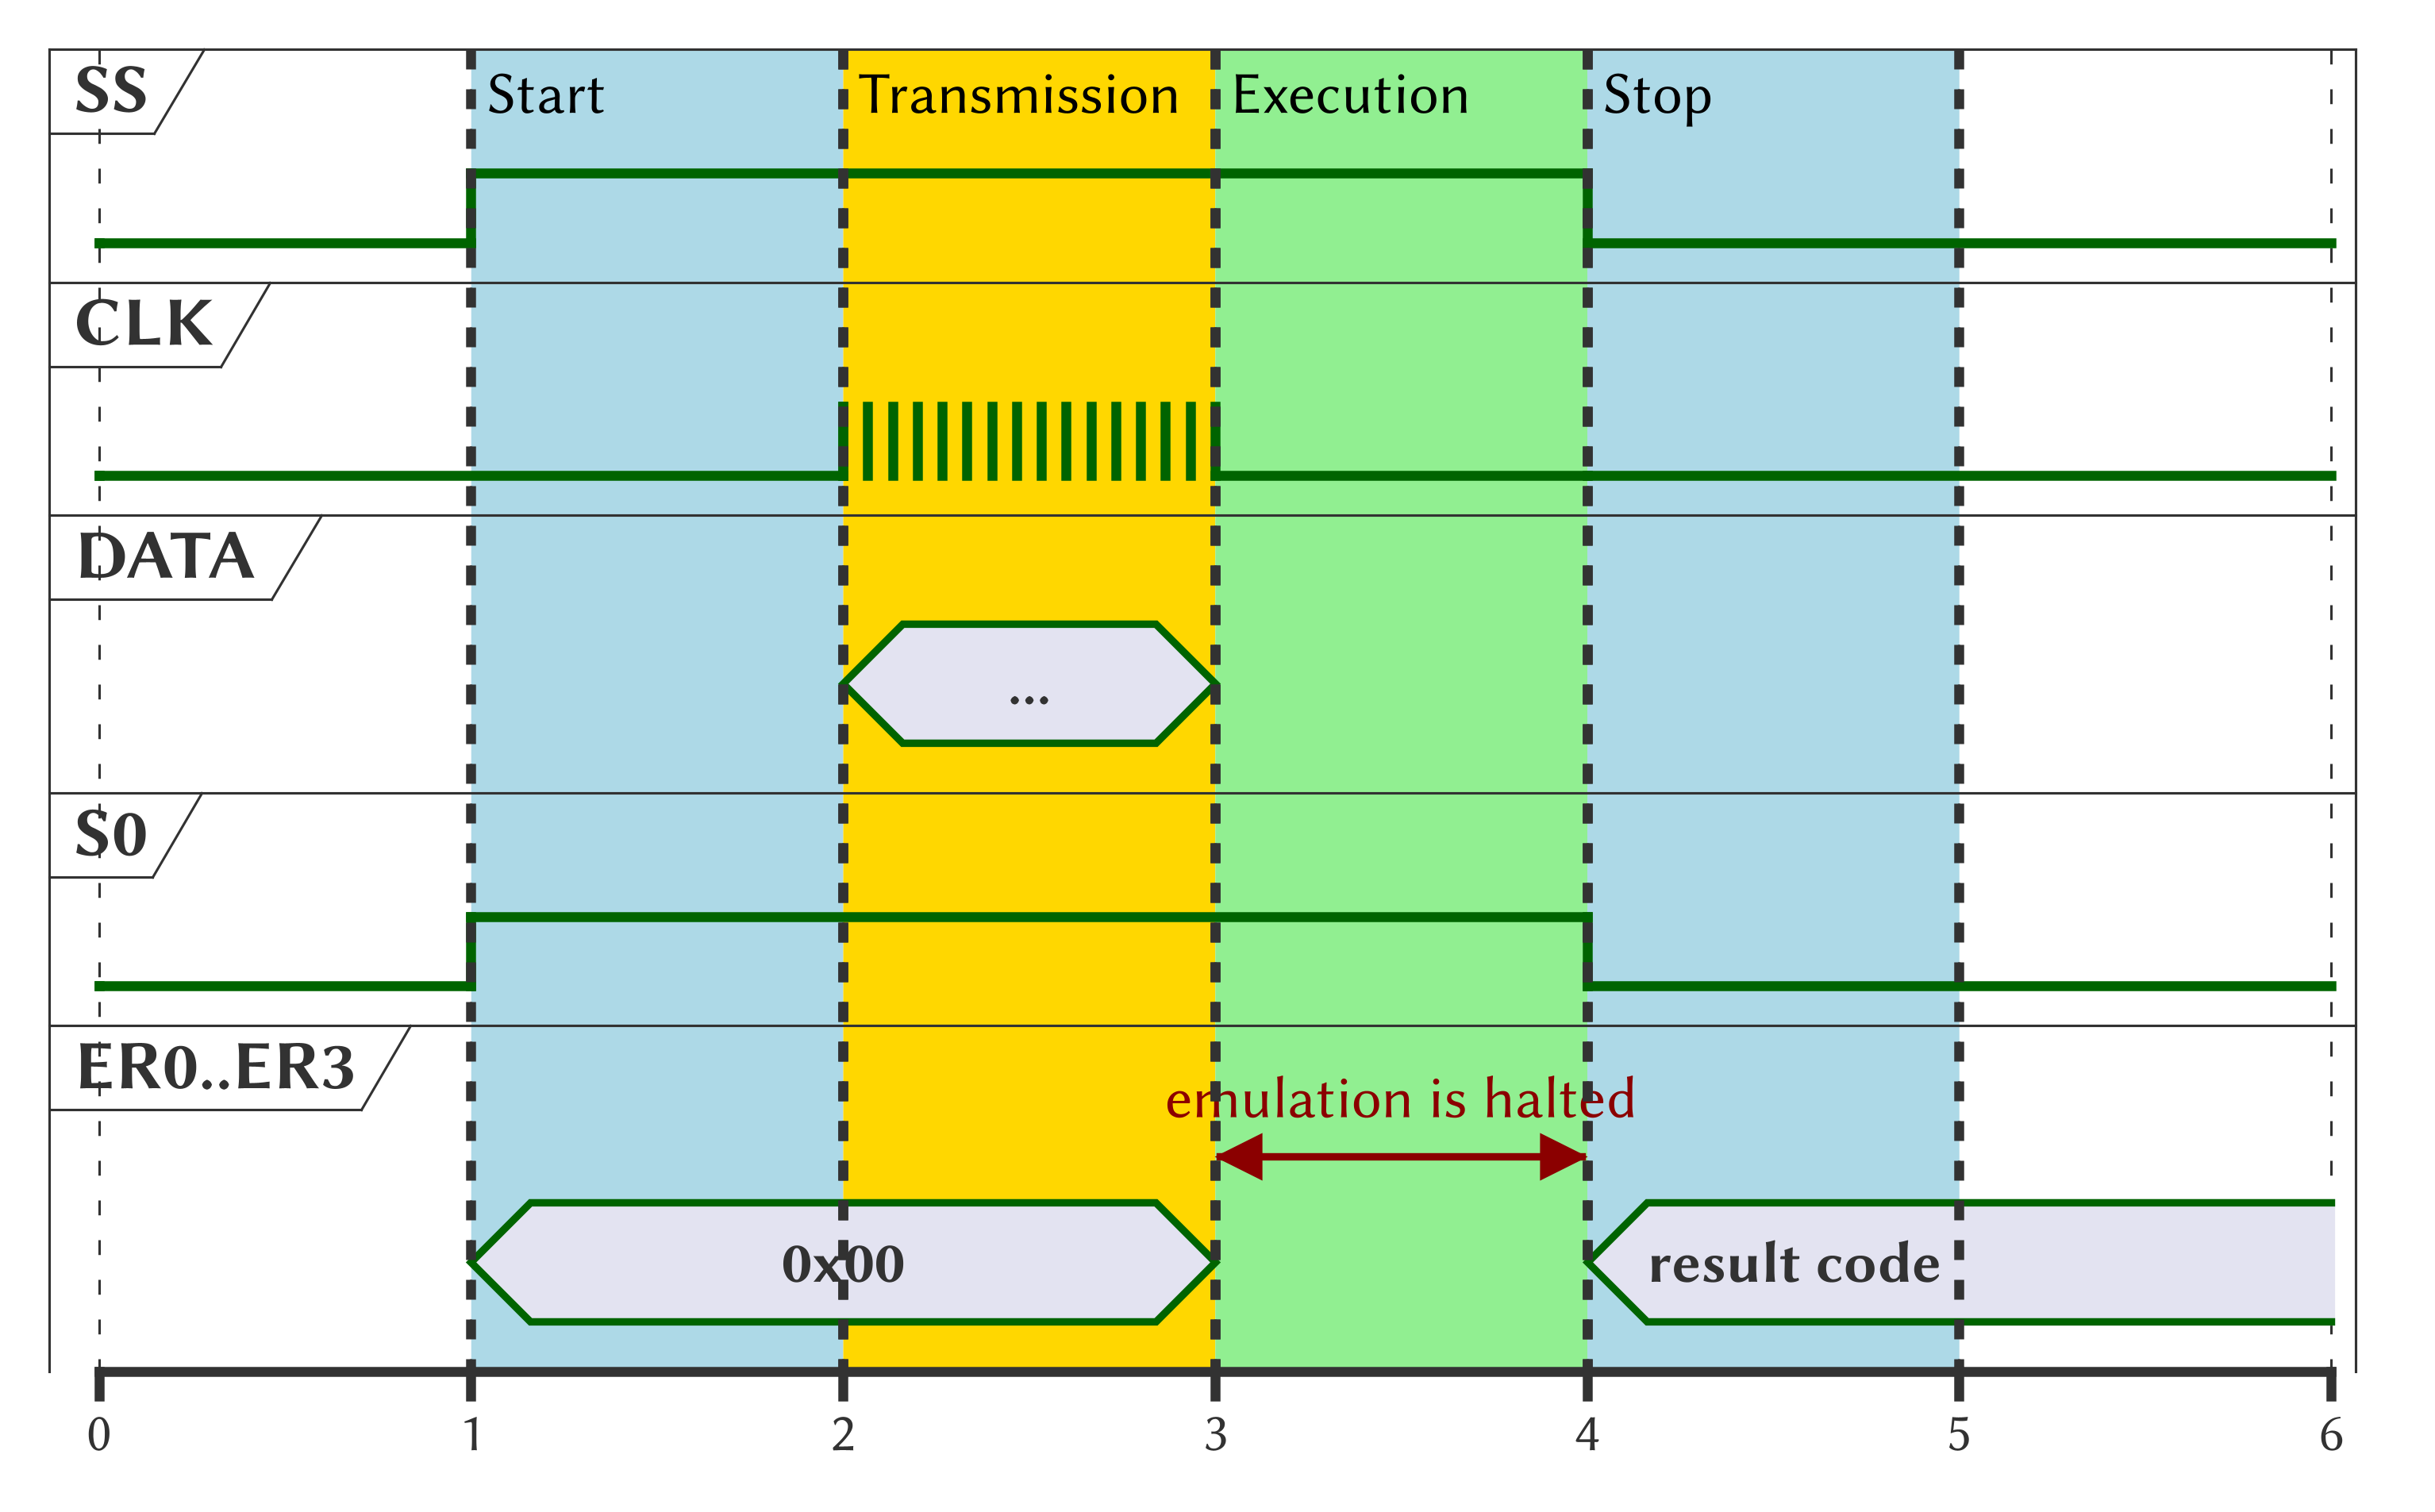
\includegraphics[width=0.9\textwidth]{soc/images/typical_communication.png}

\end{frame}

\section{BIOS}

\begin{frame}
\frametitle{BIOS}

\begin{itemize}
    \item Zabudovaný program ve \textbf{stejné formě jako ostatní NES programy}.
    \item Inicializace systému, oddělení uživatelské rozhraní a inicializační logiku od samotného
        emulátoru.
    \item Momentálně: zajišťuje načítaní programů uživatelem.
    \item V budoucnu: rozsáhlá konfigurace zařízení.
    \item \textbf{Využívá FWX pro práci s SD kartou}.
    \item Uložený na SD kartě (v budoucnu ve Flash pamětí).
\end{itemize}

\begin{columns}
    \column{0.4\textwidth}
    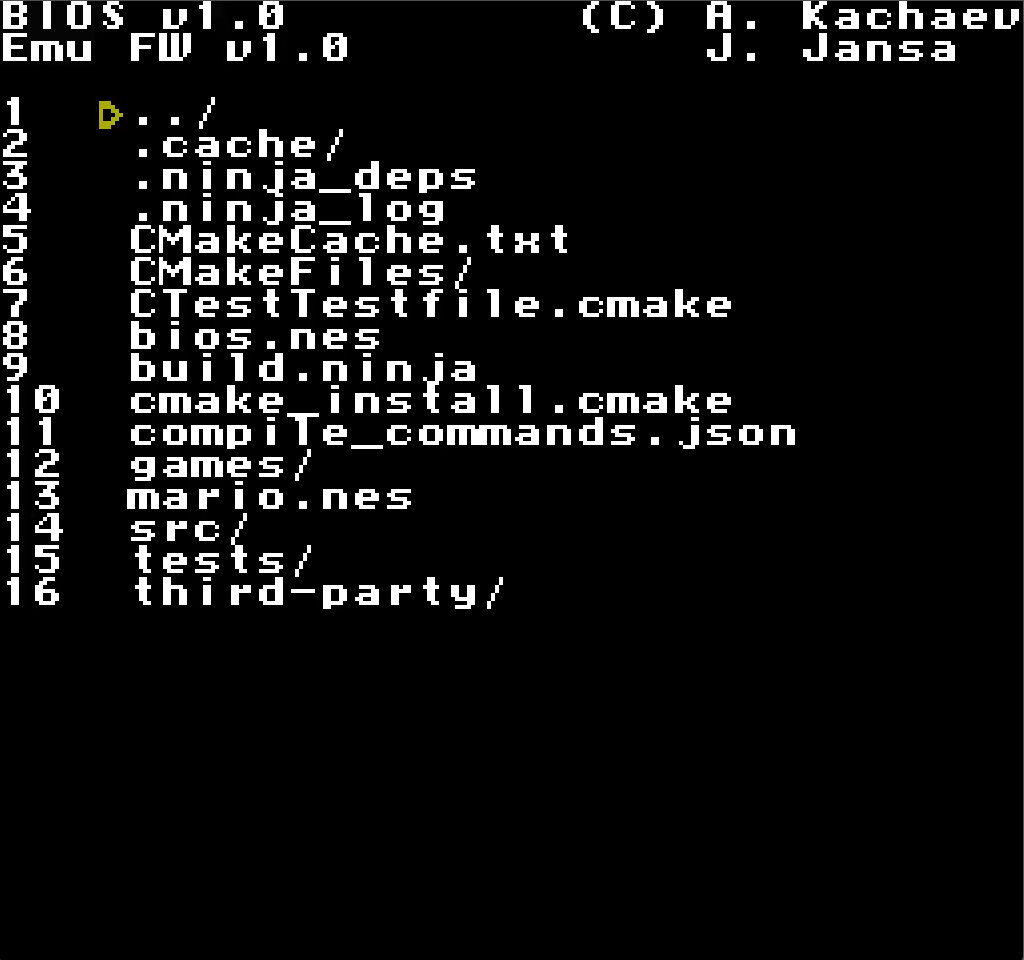
\includegraphics[width=\linewidth]{soc/images/bios.png}

    \column{0.4\textwidth}
    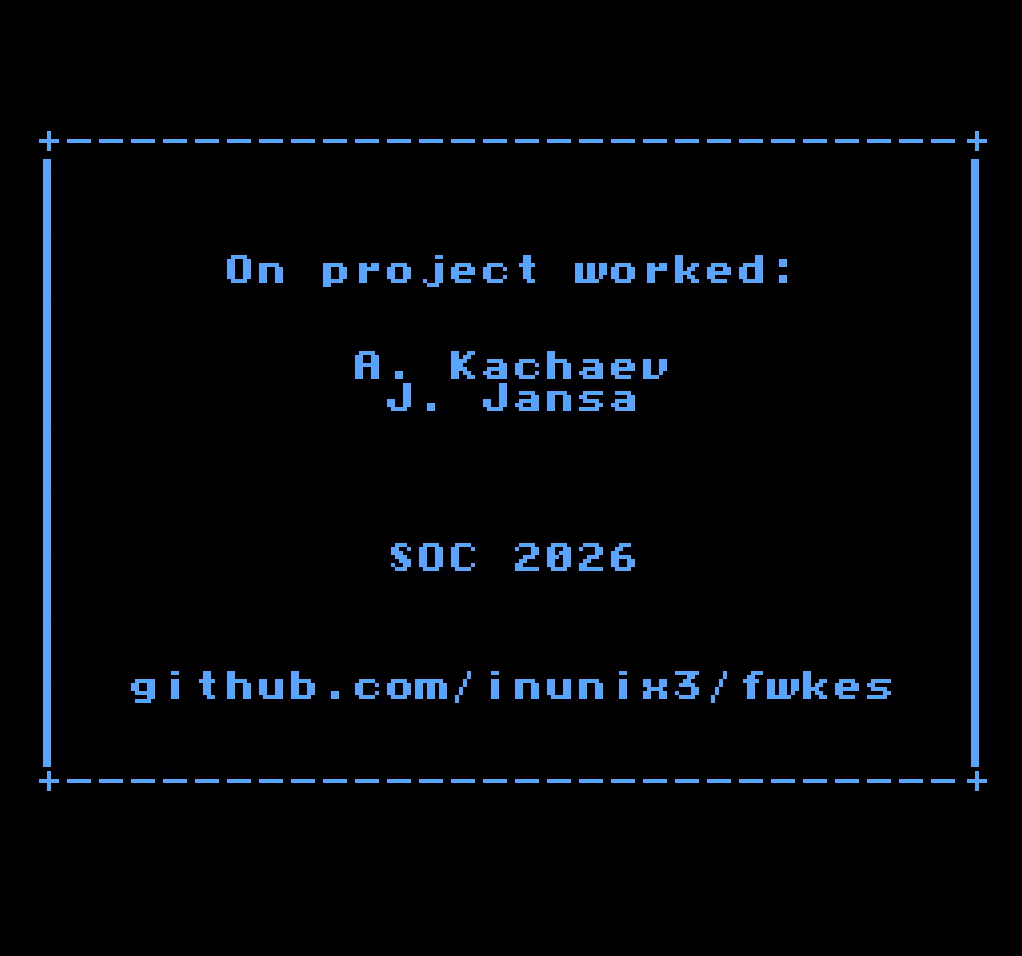
\includegraphics[width=\linewidth]{soc/images/bios_credits.png}
\end{columns}

\end{frame}

\begin{frame}
\frametitle{Hardware}

\section{Hardware}

\begin{columns}
    \column{0.4\textwidth}
    \begin{itemize}
        \item Elektrický obvod navržen v KiCad
        \item HDMI výstup, audio jack a SD karta
        \item DIN konektor pro vstupní periferie
        \item Analogový audio obvod (DAC + zesilovač)
        \item RP2350
    \end{itemize}

    \column{0.6\textwidth}
    \vspace{-2cm}
    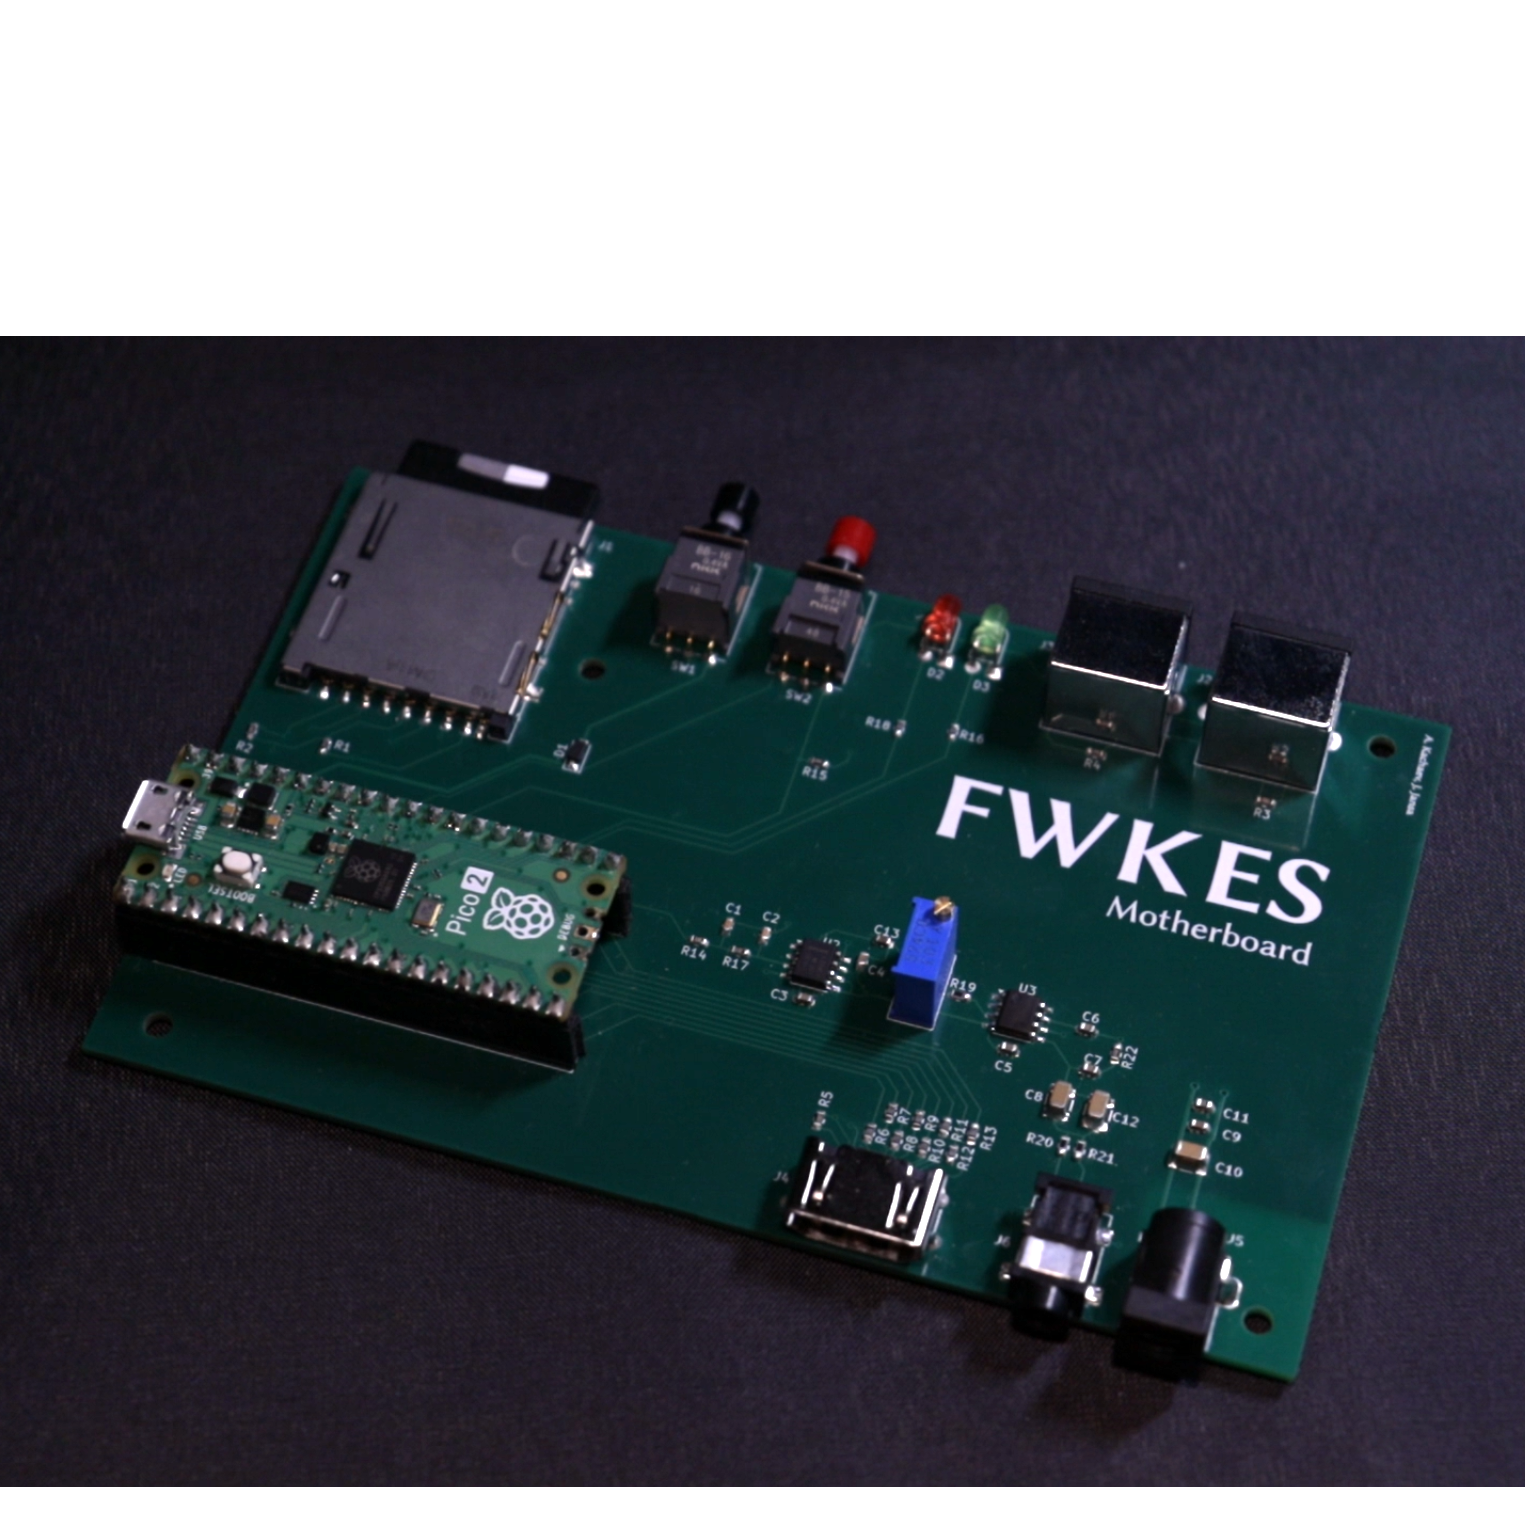
\includegraphics[width=\textwidth]{soc/images/motherboard.png}
\end{columns}

\end{frame}

\section{Závěr}

\begin{frame}
\frametitle{Závěr}

\begin{itemize}
    \item Plynulý emulátor NES na mikrokontroléru RP2350 bez OS.
    \item Komunikační rozhraní FWX pro interakci emulovaného programu a hostitelského hardwaru.
    \item Návrh a výroba zařízení.
    \item Embedded v praxi. \end{itemize}

\vspace{0.25cm}

\centering
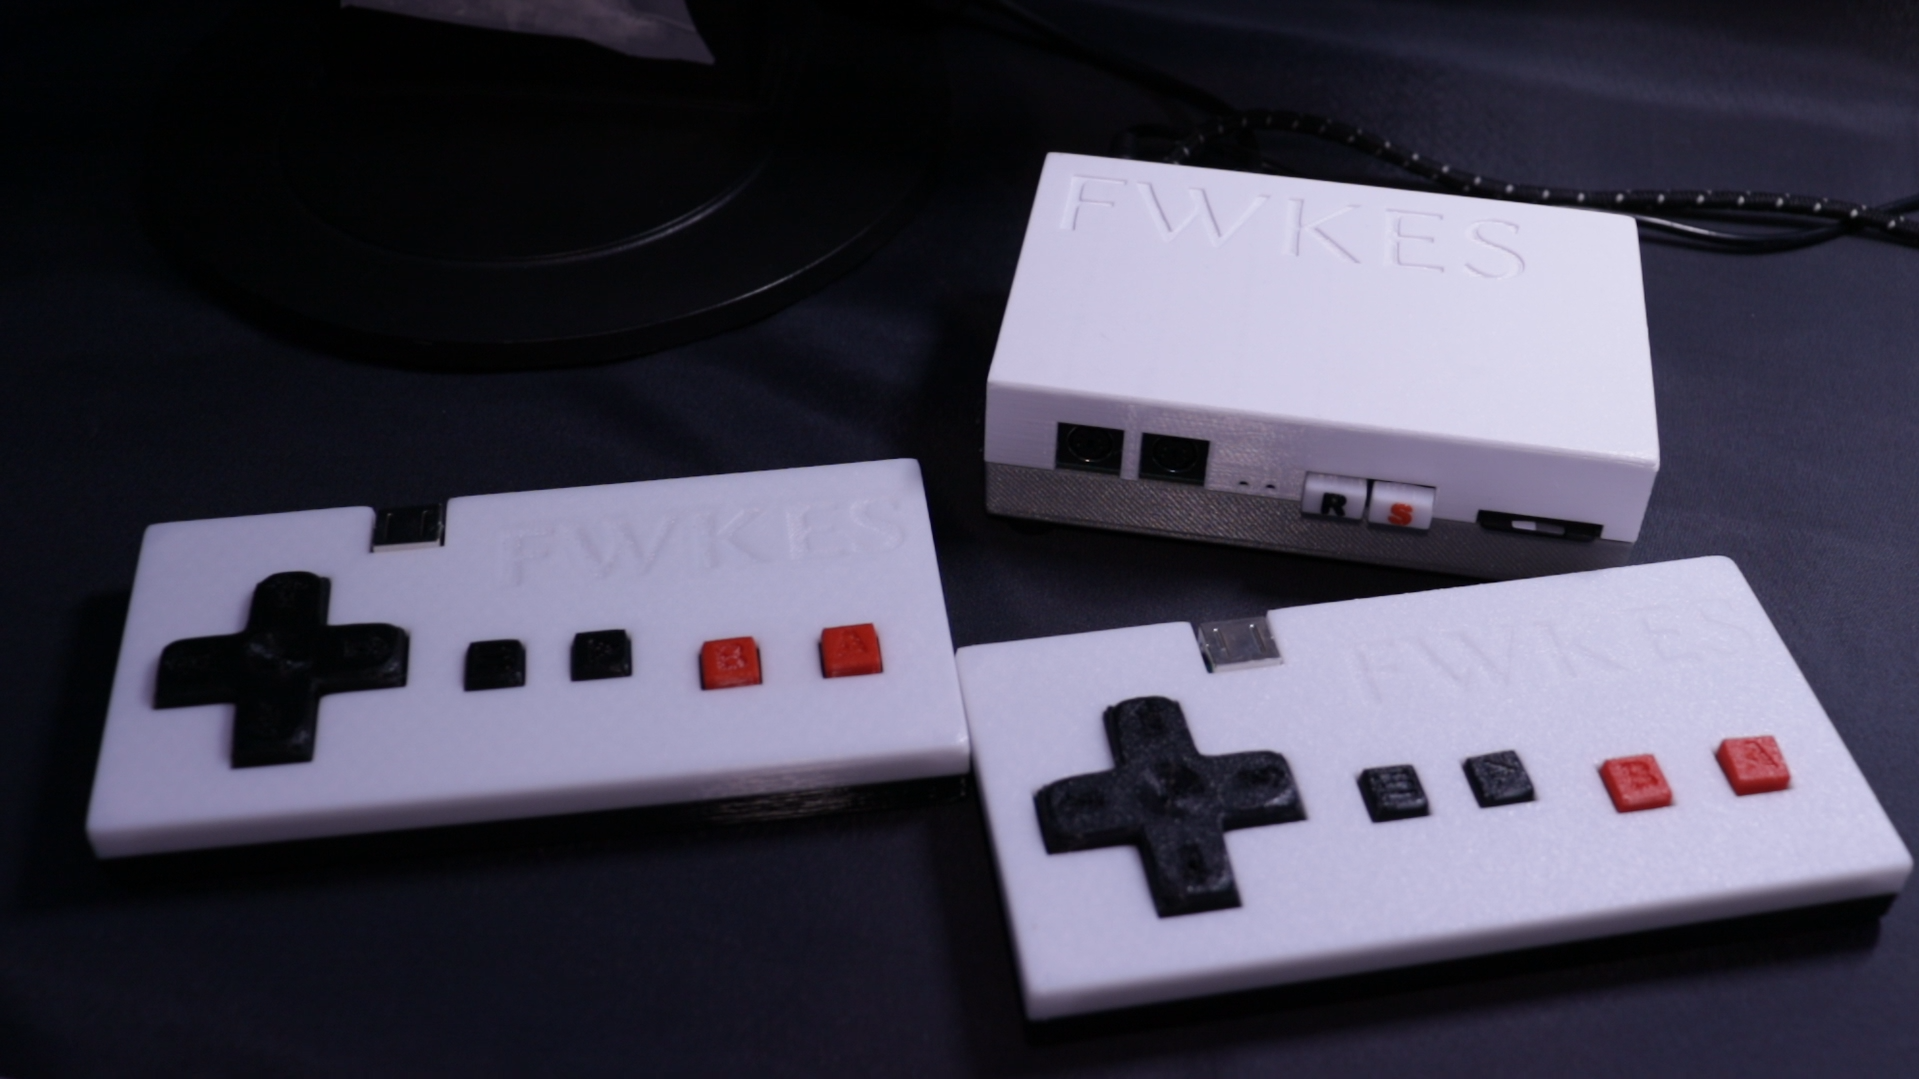
\includegraphics[width=0.75\textwidth]{soc/images/fwkes.png}

\end{frame}

\setbeamertemplate{frametitle}[default][center]

\begin{frame}
\frametitle{\LARGE Děkujeme za pozornost}

\begin{figure}
    \centering
    
\includegraphics[width=0.5\textwidth]{soc/images/hello_soc.png}
    \caption*{Snímek pořízený z našeho zařízení.}
\end{figure}

\end{frame}

\end{document}
